% Created by tikzDevice version 0.12.3 on 2020-04-10 11:40:56
% !TEX encoding = UTF-8 Unicode
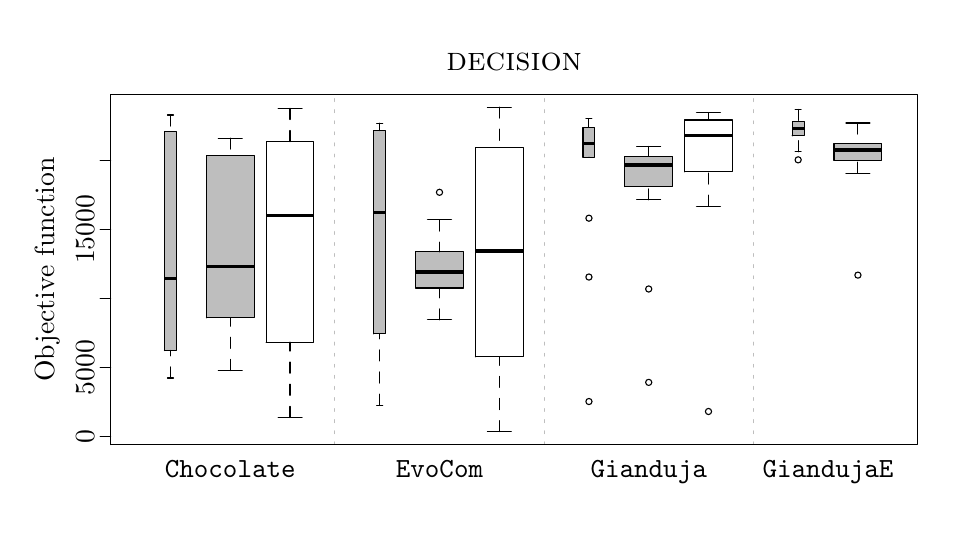
\begin{tikzpicture}[x=1pt,y=1pt]
\definecolor{fillColor}{RGB}{255,255,255}
\path[use as bounding box,fill=fillColor,fill opacity=0.00] (0,0) rectangle (325.21,180.67);
\begin{scope}
\path[clip] ( 30.00, 30.00) rectangle (321.61,156.67);
\definecolor{fillColor}{RGB}{190,190,190}

\path[fill=fillColor] ( 49.44, 64.00) --
	( 53.76, 64.00) --
	( 53.76,143.20) --
	( 49.44,143.20) --
	cycle;
\definecolor{drawColor}{RGB}{0,0,0}

\path[draw=drawColor,line width= 1.2pt,line join=round] ( 49.44, 90.01) -- ( 53.76, 90.01);

\path[draw=drawColor,line width= 0.4pt,dash pattern=on 4pt off 4pt ,line join=round,line cap=round] ( 51.60, 54.08) -- ( 51.60, 64.00);

\path[draw=drawColor,line width= 0.4pt,dash pattern=on 4pt off 4pt ,line join=round,line cap=round] ( 51.60,149.13) -- ( 51.60,143.20);

\path[draw=drawColor,line width= 0.4pt,line join=round,line cap=round] ( 50.52, 54.08) -- ( 52.68, 54.08);

\path[draw=drawColor,line width= 0.4pt,line join=round,line cap=round] ( 50.52,149.13) -- ( 52.68,149.13);

\path[draw=drawColor,line width= 0.4pt,line join=round,line cap=round] ( 49.44, 64.00) --
	( 53.76, 64.00) --
	( 53.76,143.20) --
	( 49.44,143.20) --
	( 49.44, 64.00);

\path[fill=fillColor] ( 64.56, 75.79) --
	( 81.84, 75.79) --
	( 81.84,134.63) --
	( 64.56,134.63) --
	cycle;

\path[draw=drawColor,line width= 1.2pt,line join=round] ( 64.56, 94.49) -- ( 81.84, 94.49);

\path[draw=drawColor,line width= 0.4pt,dash pattern=on 4pt off 4pt ,line join=round,line cap=round] ( 73.20, 56.79) -- ( 73.20, 75.79);

\path[draw=drawColor,line width= 0.4pt,dash pattern=on 4pt off 4pt ,line join=round,line cap=round] ( 73.20,140.78) -- ( 73.20,134.63);

\path[draw=drawColor,line width= 0.4pt,line join=round,line cap=round] ( 68.88, 56.79) -- ( 77.52, 56.79);

\path[draw=drawColor,line width= 0.4pt,line join=round,line cap=round] ( 68.88,140.78) -- ( 77.52,140.78);

\path[draw=drawColor,line width= 0.4pt,line join=round,line cap=round] ( 64.56, 75.79) --
	( 81.84, 75.79) --
	( 81.84,134.63) --
	( 64.56,134.63) --
	( 64.56, 75.79);
\definecolor{fillColor}{RGB}{255,255,255}

\path[fill=fillColor] ( 86.16, 66.99) --
	(103.44, 66.99) --
	(103.44,139.48) --
	( 86.16,139.48) --
	cycle;

\path[draw=drawColor,line width= 1.2pt,line join=round] ( 86.16,112.85) -- (103.44,112.85);

\path[draw=drawColor,line width= 0.4pt,dash pattern=on 4pt off 4pt ,line join=round,line cap=round] ( 94.80, 39.82) -- ( 94.80, 66.99);

\path[draw=drawColor,line width= 0.4pt,dash pattern=on 4pt off 4pt ,line join=round,line cap=round] ( 94.80,151.50) -- ( 94.80,139.48);

\path[draw=drawColor,line width= 0.4pt,line join=round,line cap=round] ( 90.48, 39.82) -- ( 99.12, 39.82);

\path[draw=drawColor,line width= 0.4pt,line join=round,line cap=round] ( 90.48,151.50) -- ( 99.12,151.50);

\path[draw=drawColor,line width= 0.4pt,line join=round,line cap=round] ( 86.16, 66.99) --
	(103.44, 66.99) --
	(103.44,139.48) --
	( 86.16,139.48) --
	( 86.16, 66.99);
\definecolor{fillColor}{RGB}{190,190,190}

\path[fill=fillColor] (125.04, 70.05) --
	(129.37, 70.05) --
	(129.37,143.45) --
	(125.04,143.45) --
	cycle;

\path[draw=drawColor,line width= 1.2pt,line join=round] (125.04,113.98) -- (129.37,113.98);

\path[draw=drawColor,line width= 0.4pt,dash pattern=on 4pt off 4pt ,line join=round,line cap=round] (127.20, 44.24) -- (127.20, 70.05);

\path[draw=drawColor,line width= 0.4pt,dash pattern=on 4pt off 4pt ,line join=round,line cap=round] (127.20,146.18) -- (127.20,143.45);

\path[draw=drawColor,line width= 0.4pt,line join=round,line cap=round] (126.12, 44.24) -- (128.29, 44.24);

\path[draw=drawColor,line width= 0.4pt,line join=round,line cap=round] (126.12,146.18) -- (128.29,146.18);

\path[draw=drawColor,line width= 0.4pt,line join=round,line cap=round] (125.04, 70.05) --
	(129.37, 70.05) --
	(129.37,143.45) --
	(125.04,143.45) --
	(125.04, 70.05);

\path[fill=fillColor] (140.17, 86.60) --
	(157.45, 86.60) --
	(157.45, 99.67) --
	(140.17, 99.67) --
	cycle;

\path[draw=drawColor,line width= 1.2pt,line join=round] (140.17, 92.41) -- (157.45, 92.41);

\path[draw=drawColor,line width= 0.4pt,dash pattern=on 4pt off 4pt ,line join=round,line cap=round] (148.81, 75.08) -- (148.81, 86.60);

\path[draw=drawColor,line width= 0.4pt,dash pattern=on 4pt off 4pt ,line join=round,line cap=round] (148.81,111.20) -- (148.81, 99.67);

\path[draw=drawColor,line width= 0.4pt,line join=round,line cap=round] (144.49, 75.08) -- (153.13, 75.08);

\path[draw=drawColor,line width= 0.4pt,line join=round,line cap=round] (144.49,111.20) -- (153.13,111.20);

\path[draw=drawColor,line width= 0.4pt,line join=round,line cap=round] (140.17, 86.60) --
	(157.45, 86.60) --
	(157.45, 99.67) --
	(140.17, 99.67) --
	(140.17, 86.60);

\path[draw=drawColor,line width= 0.4pt,line join=round,line cap=round] (148.81,121.18) circle (  1.12);
\definecolor{fillColor}{RGB}{255,255,255}

\path[fill=fillColor] (161.77, 61.71) --
	(179.05, 61.71) --
	(179.05,137.32) --
	(161.77,137.32) --
	cycle;

\path[draw=drawColor,line width= 1.2pt,line join=round] (161.77, 99.93) -- (179.05, 99.93);

\path[draw=drawColor,line width= 0.4pt,dash pattern=on 4pt off 4pt ,line join=round,line cap=round] (170.41, 34.69) -- (170.41, 61.71);

\path[draw=drawColor,line width= 0.4pt,dash pattern=on 4pt off 4pt ,line join=round,line cap=round] (170.41,151.98) -- (170.41,137.32);

\path[draw=drawColor,line width= 0.4pt,line join=round,line cap=round] (166.09, 34.69) -- (174.73, 34.69);

\path[draw=drawColor,line width= 0.4pt,line join=round,line cap=round] (166.09,151.98) -- (174.73,151.98);

\path[draw=drawColor,line width= 0.4pt,line join=round,line cap=round] (161.77, 61.71) --
	(179.05, 61.71) --
	(179.05,137.32) --
	(161.77,137.32) --
	(161.77, 61.71);
\definecolor{fillColor}{RGB}{190,190,190}

\path[fill=fillColor] (200.65,133.87) --
	(204.97,133.87) --
	(204.97,144.71) --
	(200.65,144.71) --
	cycle;

\path[draw=drawColor,line width= 1.2pt,line join=round] (200.65,138.76) -- (204.97,138.76);

\path[draw=drawColor,line width= 0.4pt,dash pattern=on 4pt off 4pt ,line join=round,line cap=round] (202.81,133.87) -- (202.81,133.87);

\path[draw=drawColor,line width= 0.4pt,dash pattern=on 4pt off 4pt ,line join=round,line cap=round] (202.81,147.74) -- (202.81,144.71);

\path[draw=drawColor,line width= 0.4pt,line join=round,line cap=round] (201.73,133.87) -- (203.89,133.87);

\path[draw=drawColor,line width= 0.4pt,line join=round,line cap=round] (201.73,147.74) -- (203.89,147.74);

\path[draw=drawColor,line width= 0.4pt,line join=round,line cap=round] (200.65,133.87) --
	(204.97,133.87) --
	(204.97,144.71) --
	(200.65,144.71) --
	(200.65,133.87);

\path[draw=drawColor,line width= 0.4pt,line join=round,line cap=round] (202.81, 90.56) circle (  1.12);

\path[draw=drawColor,line width= 0.4pt,line join=round,line cap=round] (202.81, 45.58) circle (  1.12);

\path[draw=drawColor,line width= 0.4pt,line join=round,line cap=round] (202.81,111.83) circle (  1.12);

\path[fill=fillColor] (215.77,123.23) --
	(233.05,123.23) --
	(233.05,134.23) --
	(215.77,134.23) --
	cycle;

\path[draw=drawColor,line width= 1.2pt,line join=round] (215.77,131.08) -- (233.05,131.08);

\path[draw=drawColor,line width= 0.4pt,dash pattern=on 4pt off 4pt ,line join=round,line cap=round] (224.41,118.44) -- (224.41,123.23);

\path[draw=drawColor,line width= 0.4pt,dash pattern=on 4pt off 4pt ,line join=round,line cap=round] (224.41,137.80) -- (224.41,134.23);

\path[draw=drawColor,line width= 0.4pt,line join=round,line cap=round] (220.09,118.44) -- (228.73,118.44);

\path[draw=drawColor,line width= 0.4pt,line join=round,line cap=round] (220.09,137.80) -- (228.73,137.80);

\path[draw=drawColor,line width= 0.4pt,line join=round,line cap=round] (215.77,123.23) --
	(233.05,123.23) --
	(233.05,134.23) --
	(215.77,134.23) --
	(215.77,123.23);

\path[draw=drawColor,line width= 0.4pt,line join=round,line cap=round] (224.41, 86.24) circle (  1.12);

\path[draw=drawColor,line width= 0.4pt,line join=round,line cap=round] (224.41, 52.50) circle (  1.12);
\definecolor{fillColor}{RGB}{255,255,255}

\path[fill=fillColor] (237.37,128.56) --
	(254.65,128.56) --
	(254.65,147.30) --
	(237.37,147.30) --
	cycle;

\path[draw=drawColor,line width= 1.2pt,line join=round] (237.37,141.76) -- (254.65,141.76);

\path[draw=drawColor,line width= 0.4pt,dash pattern=on 4pt off 4pt ,line join=round,line cap=round] (246.01,116.14) -- (246.01,128.56);

\path[draw=drawColor,line width= 0.4pt,dash pattern=on 4pt off 4pt ,line join=round,line cap=round] (246.01,149.89) -- (246.01,147.30);

\path[draw=drawColor,line width= 0.4pt,line join=round,line cap=round] (241.69,116.14) -- (250.33,116.14);

\path[draw=drawColor,line width= 0.4pt,line join=round,line cap=round] (241.69,149.89) -- (250.33,149.89);

\path[draw=drawColor,line width= 0.4pt,line join=round,line cap=round] (237.37,128.56) --
	(254.65,128.56) --
	(254.65,147.30) --
	(237.37,147.30) --
	(237.37,128.56);

\path[draw=drawColor,line width= 0.4pt,line join=round,line cap=round] (246.01, 41.98) circle (  1.12);
\definecolor{fillColor}{RGB}{190,190,190}

\path[fill=fillColor] (276.25,141.60) --
	(280.57,141.60) --
	(280.57,146.74) --
	(276.25,146.74) --
	cycle;

\path[draw=drawColor,line width= 1.2pt,line join=round] (276.25,144.33) -- (280.57,144.33);

\path[draw=drawColor,line width= 0.4pt,dash pattern=on 4pt off 4pt ,line join=round,line cap=round] (278.41,135.84) -- (278.41,141.60);

\path[draw=drawColor,line width= 0.4pt,dash pattern=on 4pt off 4pt ,line join=round,line cap=round] (278.41,151.14) -- (278.41,146.74);

\path[draw=drawColor,line width= 0.4pt,line join=round,line cap=round] (277.33,135.84) -- (279.49,135.84);

\path[draw=drawColor,line width= 0.4pt,line join=round,line cap=round] (277.33,151.14) -- (279.49,151.14);

\path[draw=drawColor,line width= 0.4pt,line join=round,line cap=round] (276.25,141.60) --
	(280.57,141.60) --
	(280.57,146.74) --
	(276.25,146.74) --
	(276.25,141.60);

\path[draw=drawColor,line width= 0.4pt,line join=round,line cap=round] (278.41,132.91) circle (  1.12);

\path[fill=fillColor] (291.37,132.72) --
	(308.65,132.72) --
	(308.65,138.85) --
	(291.37,138.85) --
	cycle;

\path[draw=drawColor,line width= 1.2pt,line join=round] (291.37,136.42) -- (308.65,136.42);

\path[draw=drawColor,line width= 0.4pt,dash pattern=on 4pt off 4pt ,line join=round,line cap=round] (300.01,128.09) -- (300.01,132.72);

\path[draw=drawColor,line width= 0.4pt,dash pattern=on 4pt off 4pt ,line join=round,line cap=round] (300.01,146.23) -- (300.01,138.85);

\path[draw=drawColor,line width= 0.4pt,line join=round,line cap=round] (295.69,128.09) -- (304.33,128.09);

\path[draw=drawColor,line width= 0.4pt,line join=round,line cap=round] (295.69,146.23) -- (304.33,146.23);

\path[draw=drawColor,line width= 0.4pt,line join=round,line cap=round] (291.37,132.72) --
	(308.65,132.72) --
	(308.65,138.85) --
	(291.37,138.85) --
	(291.37,132.72);

\path[draw=drawColor,line width= 0.4pt,line join=round,line cap=round] (300.01, 91.25) circle (  1.12);
\definecolor{drawColor}{RGB}{190,190,190}

\path[draw=drawColor,line width= 0.4pt,dash pattern=on 1pt off 3pt ,line join=round,line cap=round] (111.00, 30.00) -- (111.00,156.67);

\path[draw=drawColor,line width= 0.4pt,dash pattern=on 1pt off 3pt ,line join=round,line cap=round] (186.61, 30.00) -- (186.61,156.67);

\path[draw=drawColor,line width= 0.4pt,dash pattern=on 1pt off 3pt ,line join=round,line cap=round] (262.21, 30.00) -- (262.21,156.67);
\end{scope}
\begin{scope}
\path[clip] (  0.00,  0.00) rectangle (325.21,180.67);
\definecolor{drawColor}{RGB}{0,0,0}

\node[text=drawColor,anchor=base,inner sep=0pt, outer sep=0pt, scale=  1.00] at ( 73.20, 18.00) {\texttt{Chocolate}};

\node[text=drawColor,anchor=base,inner sep=0pt, outer sep=0pt, scale=  1.00] at (148.81, 18.00) {\texttt{EvoCom}};

\node[text=drawColor,anchor=base,inner sep=0pt, outer sep=0pt, scale=  1.00] at (224.41, 18.00) {\texttt{Gianduja}};

\node[text=drawColor,anchor=base,inner sep=0pt, outer sep=0pt, scale=  1.00] at (289.21, 18.00) {\texttt{GiandujaE}};
\end{scope}
\begin{scope}
\path[clip] (  0.00,  0.00) rectangle (325.21,180.67);
\definecolor{drawColor}{RGB}{0,0,0}

\node[text=drawColor,anchor=base,inner sep=0pt, outer sep=0pt, scale=  1.20] at (175.81,165.07) {\textsc{decision}};

\node[text=drawColor,rotate= 90.00,anchor=base,inner sep=0pt, outer sep=0pt, scale=  1.00] at (  9.60, 93.34) {Objective function};
\end{scope}
\begin{scope}
\path[clip] (  0.00,  0.00) rectangle (325.21,180.67);
\definecolor{drawColor}{RGB}{0,0,0}

\path[draw=drawColor,line width= 0.4pt,line join=round,line cap=round] ( 30.00, 32.88) -- ( 30.00,132.81);

\path[draw=drawColor,line width= 0.4pt,line join=round,line cap=round] ( 30.00, 32.88) -- ( 26.20, 32.88);

\path[draw=drawColor,line width= 0.4pt,line join=round,line cap=round] ( 30.00, 57.86) -- ( 26.20, 57.86);

\path[draw=drawColor,line width= 0.4pt,line join=round,line cap=round] ( 30.00, 82.84) -- ( 26.20, 82.84);

\path[draw=drawColor,line width= 0.4pt,line join=round,line cap=round] ( 30.00,107.82) -- ( 26.20,107.82);

\path[draw=drawColor,line width= 0.4pt,line join=round,line cap=round] ( 30.00,132.81) -- ( 26.20,132.81);

\node[text=drawColor,rotate= 90.00,anchor=base,inner sep=0pt, outer sep=0pt, scale=  1.00] at ( 24.00, 32.88) {0};

\node[text=drawColor,rotate= 90.00,anchor=base,inner sep=0pt, outer sep=0pt, scale=  1.00] at ( 24.00, 57.86) {5000};

\node[text=drawColor,rotate= 90.00,anchor=base,inner sep=0pt, outer sep=0pt, scale=  1.00] at ( 24.00,107.82) {15000};

\path[draw=drawColor,line width= 0.4pt,line join=round,line cap=round] ( 30.00, 30.00) --
	(321.61, 30.00) --
	(321.61,156.67) --
	( 30.00,156.67) --
	( 30.00, 30.00);
\end{scope}
\end{tikzpicture}
